\chapter{РЕАЛІЗАЦІЯ ПРОГРАМНОГО ЗАБЕЗПЕЧЕННЯ ДОДАТКУ}

\section{Архітектура додатку}
Введемо наступні поняття:

\begin{itemize}
\item \textbf{Event} (подія) - деяка подія, на яку додаток повинен відреагувати, наприклад - нове повідомлення від користувача.
\item \textbf{Action} (реакція) - реакція додатку на подію, наприклад - збереження нагадування у базу.
\item \textbf{Environment} (середовище) - джерело подій.
\item \textbf{Context} (контекст) - набір даних, об'єднаних за деякою ознакою.
\item \textbf{User} (користувач) - користувач нашого додатку.
\end{itemize}

Побудуємо додаток наступним чином: нехай маємо деякий набір середовищ. Додаток у нескінченому циклі по черзі питає в кожного середовища нові події та реагує на них. Додаток може реагувати на події як окремо, так і будувати певні реакції в залежності від набору подій. 


При першій інтеракції користувача з додатком йому присвоїться унікальний ідентифікатор. Ми зберігатимемо усі дані користувача, що він надав (історію повідомлень, факти надані користувачем, тощо) для того щоб мати можливість персоналізувати його взаємодію з ботом[22]. У подальшому, при визначенні реакції на подію ми враховуватимемо також контекст користувача - тобто сукупність даних про нього.


Таким чином, додаток досить легко розширювати в усі сторони, оскільки усі частини є достатньо незалежними. Якщо ми хочемо додати нову функцію, нам потрібно лише описати подію та відповідну їй реакцію, тобто дію. Якщо ми хочемо зберігати більше даних, нам достатньо лише розширити відповідні контексти. Якщо ми хочемо додати нову платформу, нам достатньо лише вказати яким саме чином ми будемо отримувати повідомлення про дії з неї та задати необхідні реакції. 
\section{Реалізація боту}
Бот складається з чотирьох мікросервісів:
\begin{enumerate}
\item Основний сервіс, написаний мовою Scala - який відповідає за роботу бота
\item Допоміжний сервіс, написаний мовою Scala - використовується разом з SparkNLP для визначення іменованих сутностей у тексті.
\item Сервіс на Python - дає доступ до моделі, що визначає тип повідомлення.
\item Сервіс на Python  - дає доступ до моделі BERT.
\end{enumerate}

Спілкування між сервісами відбувається за допомогою HTTP - повідомлень. Бот також використовує базу даних для зберігання інформації про користувачів. Датасети записуються у текстові файли, що зберігаються на сервері.
\subsection{Месенджер}
У якості месенджера для спілкування з асистентом я обрав Telegram через відносну простоту налаштування та запуску боту. Такий вибір платформи дає можливість в подальшому розширити бота на спілкування не лише текстом, а й за допомогою відеоповідомлень, зображень чи аудіоповідомлень. Для спілкування з API Telegram було обрано існуючу бібліотеку bot4s. 

Відповідно до архітектури, маємо середовище Telegram, яке у якості подій надсилає нам нові повідомлення від користувачів. Бот у свою чергу реагує на них - відповідає іншим повідомленням, оновлює інформацію про користувача, робить запити на зовнішні API чи інші сервіси. Крім того, усі повідомлення логуються у окремий датасет. що дає змогу після анотування використовувати повідомлення для тренування власних моделей.
\subsection{Розпізнавання типу повідомлення}
Для того, щоб якісніше оброблювати повідомлення, необхідно знати, якого саме воно типу.  Введемо 4 наступні типи повідомлень:
\begin{center}
\begin{tabular}{ |c|c| } 
 \hline
Тип повідомлення & Приклад\\
Питання & “What is my age?”\\
Факт & “I am 20 years old”\\
Запит & “Remind me to drink water tomorrow”\\
Інше & “Hello!"\\
 \hline
\end{tabular}
\end{center}\\
\textit{таб. 1 Типи повідомлень.}


Проблема полягає в тому, що не всі користувачі правильно ставлять розділові знаки, тому "what is my age"  має отримати таку саму реакцію від бота, як і "what is my age?". З іншого боку, для запитів, що потребують зовнішні дані (наприклад, "what is the weather today?") цілком нормально мати знак питання, але бути кваліфікованим як саме запит.


Зібравши датасет з повідомлень, та проанотувавши його вручну, натренуємо власний класифікатор повідомлень. Для датасету проводилась така передобробка:

\begin{enumerate}
\item Токенізація (розбиття тексту на слова)
\item Видалення «стоп-слів» (слів, які зазвичай використовуються дуже часто і псують якість моделі)
\item Використання підходу “мішок слів” для переведення слів у числову характеристику.
\end{enumerate}
Найпростіший класифікатор, що тим не менш видає непогану точність, натренуємо наступним чином:

\begin{enumerate}
\item Закодуємо повідомлення за допомогою методу bag of words.
\item Порахуємо кількість знаків запитань у повідомленні.
\item Порахуємо кількість так званих wh-words в повідомленні.
\item Враховуватимемо перше слово у повідомленні окремо.
\item На основі вищевказаних даних натренуємо класифікатор на базі дерева рішень.
\end{enumerate}
На зібраному датасеті отримуємо точність 91.1\%, що є досить непоганою точністю, враховуючи невеликий розмір датасету.

\subsection{Нагадування}
Якщо бот розпізнає повідомлення як запит,  і у тексті міститься ключове слово remind, бот відреагує на повідомлення - перепитає, чи правильно він зрозумів користувача про що і коли потрібно нагадати. Таким чином, збирається датасет нагадувань, на якому можна натренувати модель, що буде відповідати на питання "про що саме потрібно нагадати". Для витягування "тіла" нагадування використовується модель BERT, якій на вхід у якості тексту дається повідомлення, а у якості питання - "What should I remind you about?". На невеликому зібранному датасеті нагадувань BERT дає точність 100\%.\\
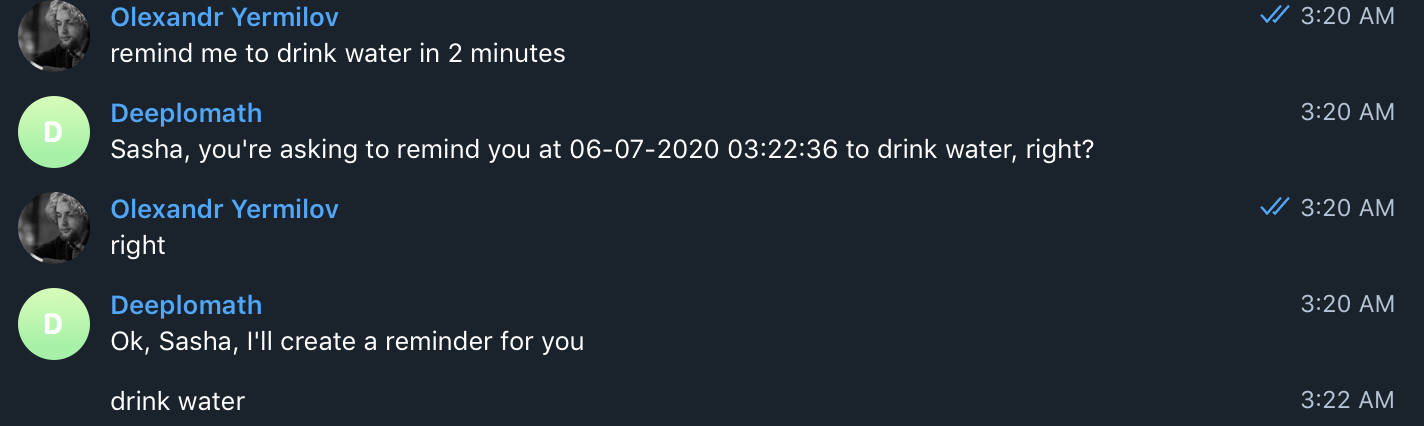
\includegraphics[width=500]{Dissertation/reminder_working.png}.\\
\textit{рис 7. Приклад роботи нагадування.}


Для визначення часу нагадування ми можемо парсити повідомлення користувача, або поєднювати BERT та роботу сервісу. Як і на питання "Про що необхідно нагадати", модель BERT може відповісти на питання "Коли потрібно нагадати?". Але необхідно враховувати, що модель може лише витягнути дані з запиту користувача, і аж ніяк не може дати точний час, у який потрібно нагадати, оскільки модель нічого не знає про те, котра зараз година.\\ 
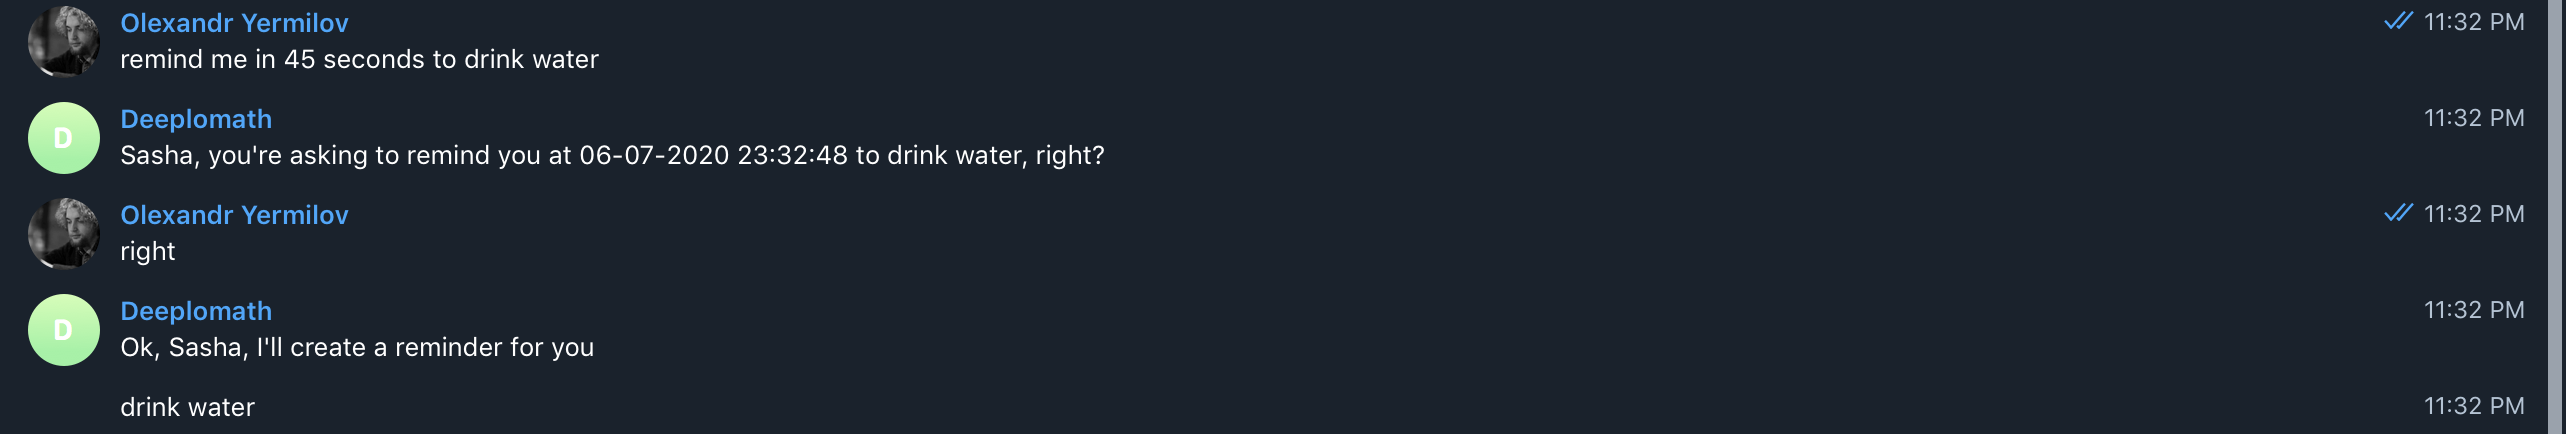
\includegraphics[width=500]{Dissertation/remind_seconds.png}.\\
\textit{рис. 8. Нагадування з іншою одиницею виміру часу.}

\subsection{Запити на зовнішні сервіси}
Робота будь-якого чат-бота сильно залежить від функцій, які він вміє виконувати по запиту користувача. Одним з найкращих способів розширювати його функціональність є інтеграція зі сторонніми API та сервісами, які надають різну інформацію.  

\subsubsection{YahooFinance}
Бот зінтегровано з  API від YahooFinance, що дозволяє дізнаватись ціну акції конкретної компанії. Логіка обробки повідомлення схожа на логіку обробки запиту про нагадування - класифікували повідомлення як запит, за допомогою моделі BERT дістали назву компанії, ціна акцій якої нас цікавить, та виконали запит до стороннього сервісу.\\
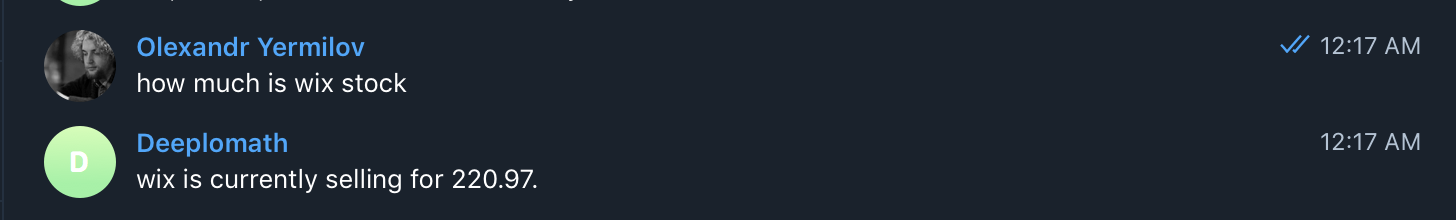
\includegraphics[width=500]{Dissertation/stocks_working.png}.\\
\textit{рис 9. Приклад роботи  запиту на сторонній сервіс.}


Крім того, знаючи запити користувача наприклад щодо акцій певної компанії, можемо вважати що він має певний інтерес до неї. Тобто, зберігаючи інформацію такого роду, можна персоналізувати досвід користувача - наприклад, через деякий час запитати, чи цікаво йому знову отримати інформацію про дану компанію. Такого роду інформація зберігається у контексті користувача як інтереси. \\
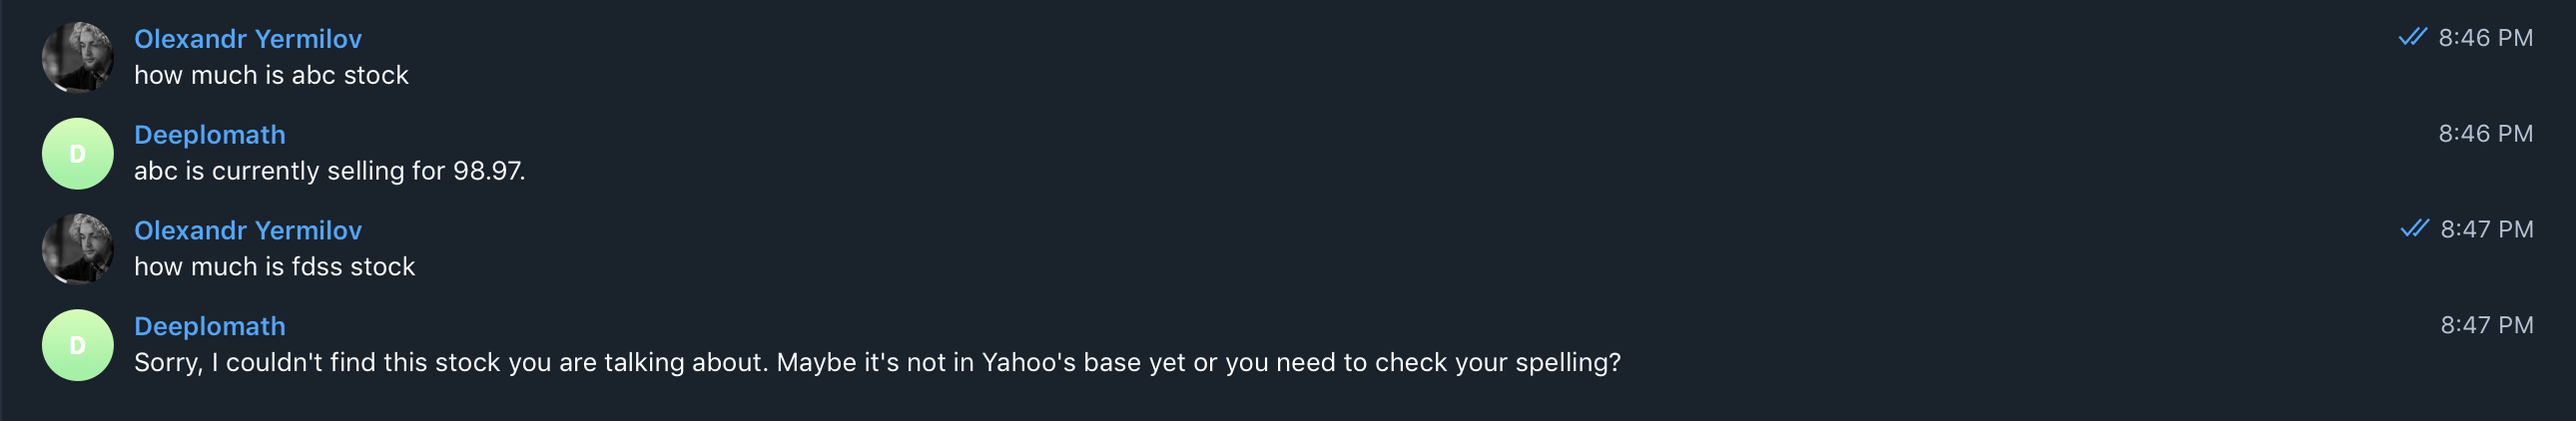
\includegraphics[width = 500]{Dissertation/stocks_not_working.png}\\
\textit{рис. 10 Кілька прикладів роботи з цінами на акції.}


\subsubsection{FoodApi}
Іншим сервісом, обраним для інтеграції з додатком, є сервіс FoodApi. Він дозволяє дізнаватися просту інформацію про їжу - калорії, корисність та склад, тощо. Даний сервіс автоматично відповідає на питання, тому єдине що необхідно зрозуміти - чи повідомлення є запитанням про їжу, чи ні.
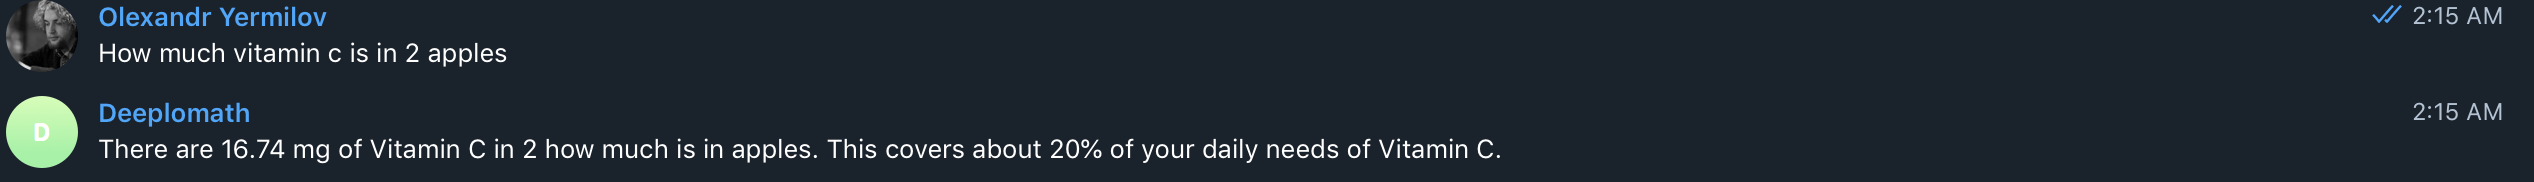
\includegraphics[width = 500]{Dissertation/food_api.png}\\
\textit{рис. 11 Приклад запиту про їжу}\\
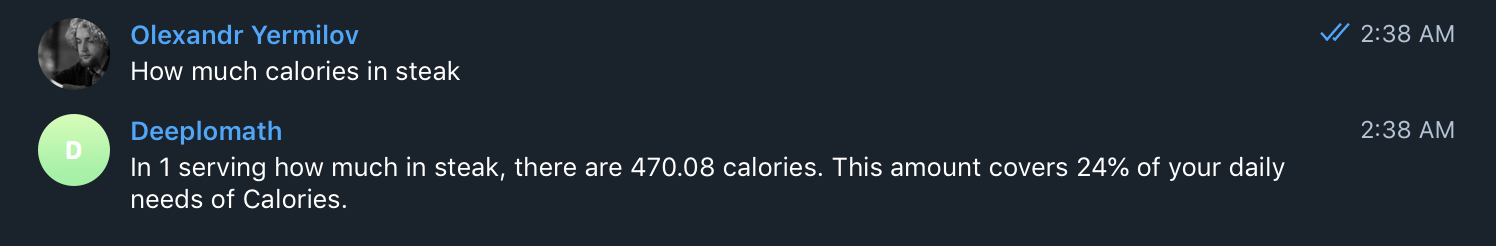
\includegraphics[width = 500]{Dissertation/foodapi2.png}\\
\textit{рис. 12 Запит калорій.}

\subsubsection{Weather API}

Одним із можливо найпопулярніших запитів у чат-ботах є "яка зараз погода?". Для визначення точної погоди необхідно знати точні координати місця, про яке запитує користувач. Для цього можна скористатись стороннім API від Google Maps. 

Для того, щоб дізнатись, про яке саме місце говорить користувач, за звичною схемою запитаємо про це у моделі BERT. Текстом буде питання користувача, у якості питання - "where?" \\
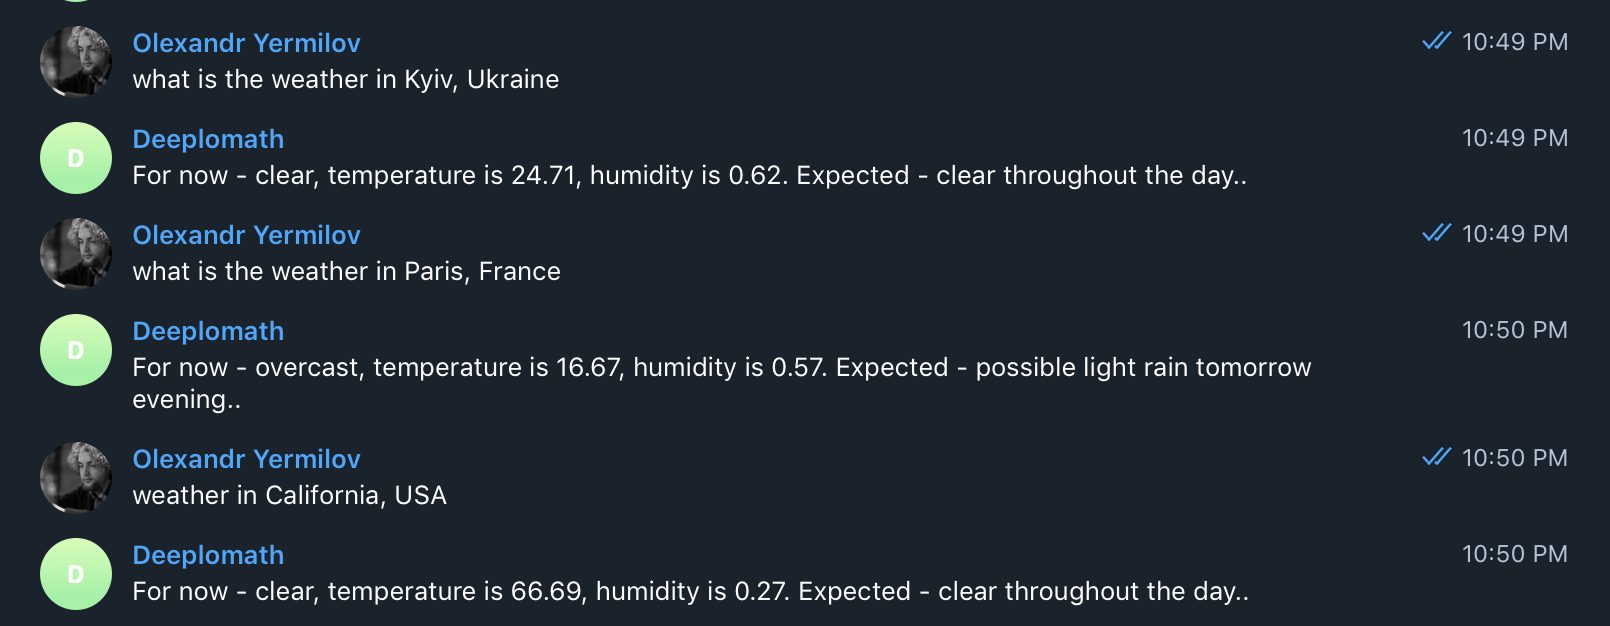
\includegraphics[width = 450]{Dissertation/weather1.png}\\
\textit{рис. 13. Приклад запитів про погоди у різних містах.}

Для визначення погоди скористаємося такоє стороннім API, передавши у якості параметрів довготу та широту місця, про яке запитував користувач. Отримаємо короткий опис теперішнього стану погоди та прогноз на найближчий час. \\
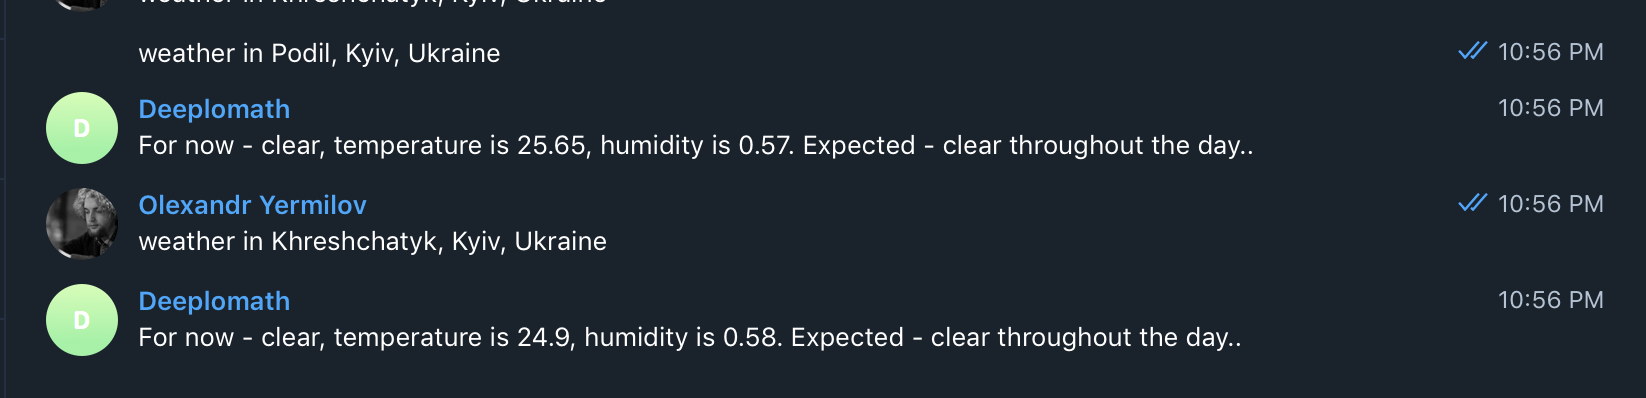
\includegraphics[width = 450]{Dissertation/weather2.png}\\
\textit{рис. 14. Приклад запиту погоди у конкретному районі.}

Як бачимо, завдяки точному визначенню координат можемо отримувати дані про погоду у різних частина Києва.

Телеграм також має підтримку надсилання координат на карті. Скористаємося ними для перевірки погоди за положенням користувача:\\
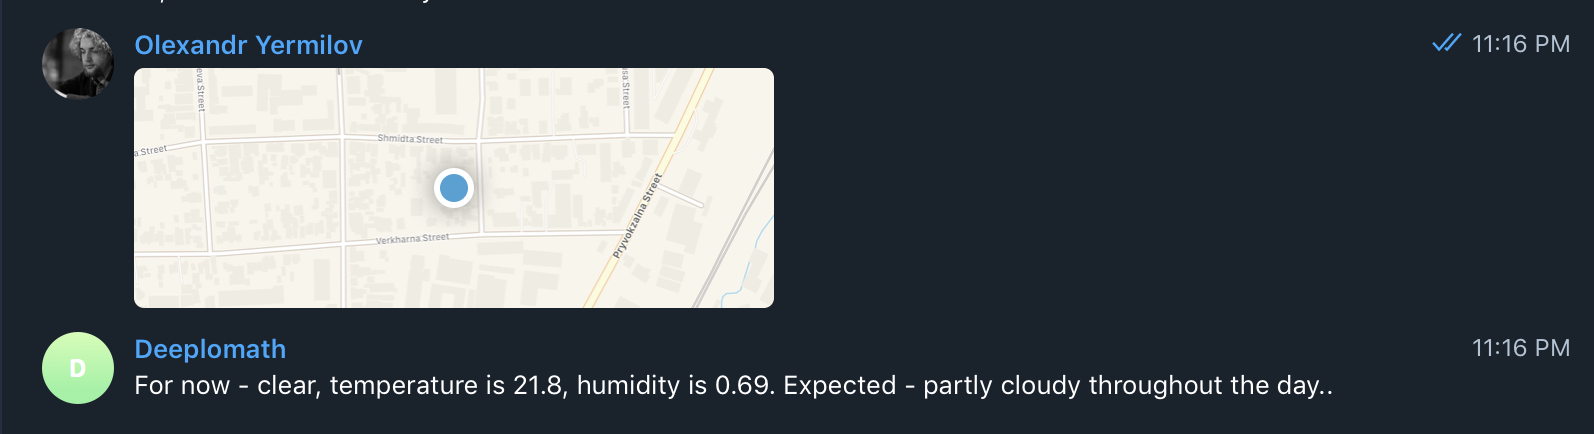
\includegraphics[width = 450]{Dissertation/weather3.png}\\
\textit{рис. 15. Приклад запиту за координатами користувача.}

\subsubsection{COVID API}
Додамо актуальний на даний момент запит - статистика по кількості захворівших COVID-19 у різних країнах. Як зазвичай, скористаємося BERT для визначення країни з запитання користувача за допомогою запитання "where?" та стороннім API для отримання статистики.\\
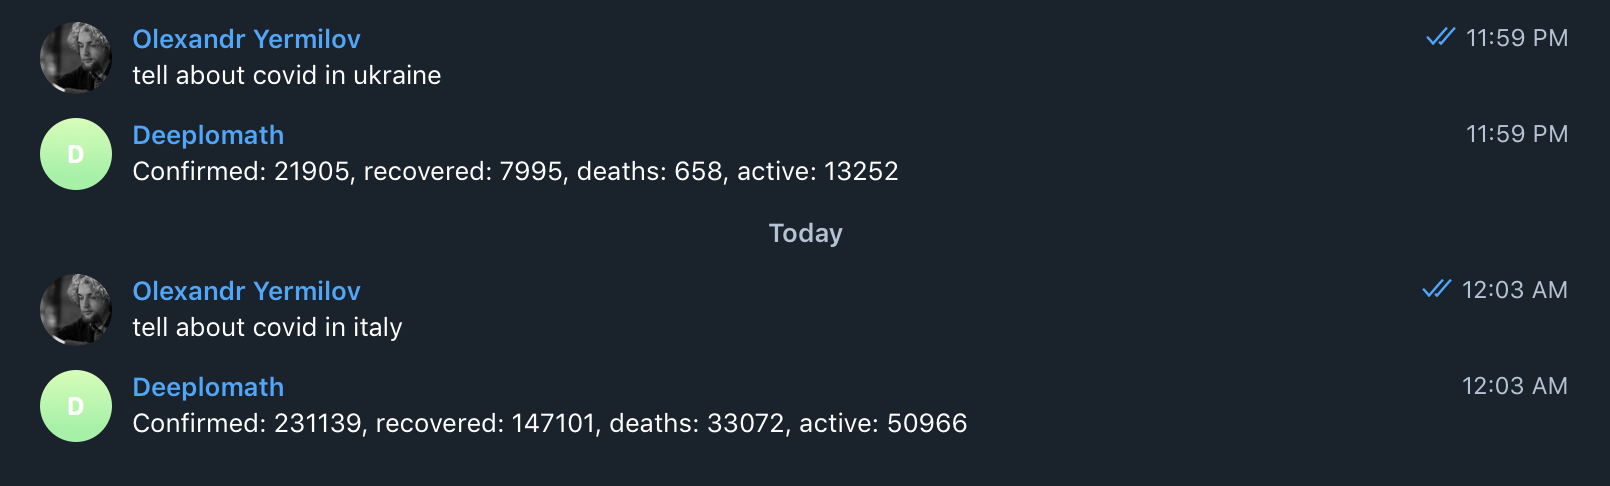
\includegraphics[width = 450]{Dissertation/covid.png}\\
\textit{рис. 16. Приклад запиту про COVID-19}
 

\subsection{Тон повідомлення}
Тон повідомлення є важливою інформацією - якщо користувач протягом останнього часу звучить занадто сумно, це може свідчити про певні проблеми у нього. За допомогою моделі Sentiment Analysis маємо змогу оцінювати кожне повідомлення користувача від -1 до 1, зберігати це значення, після чого у випадку якщо середнє значення перейде за певну межу, можемо зробити висновок про настрій користувача.\\
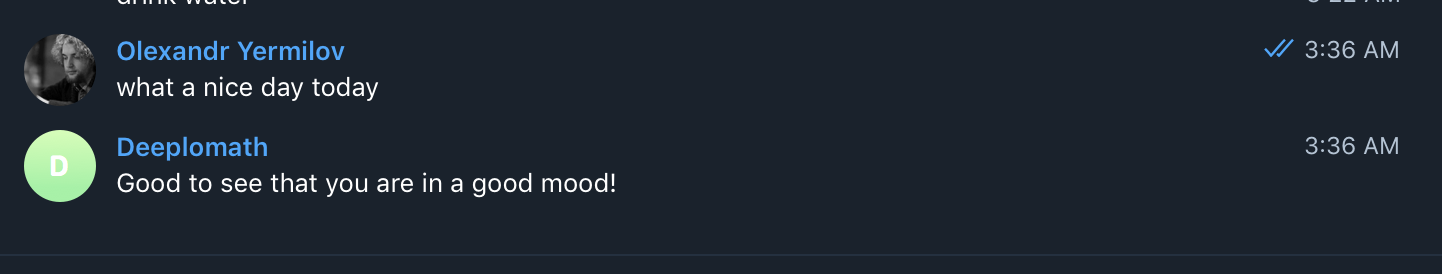
\includegraphics[width=500]{Dissertation/good_sent.png}.\\
\textit{рис. 17. Приклад реакції на гарний настрій користувача.}\\
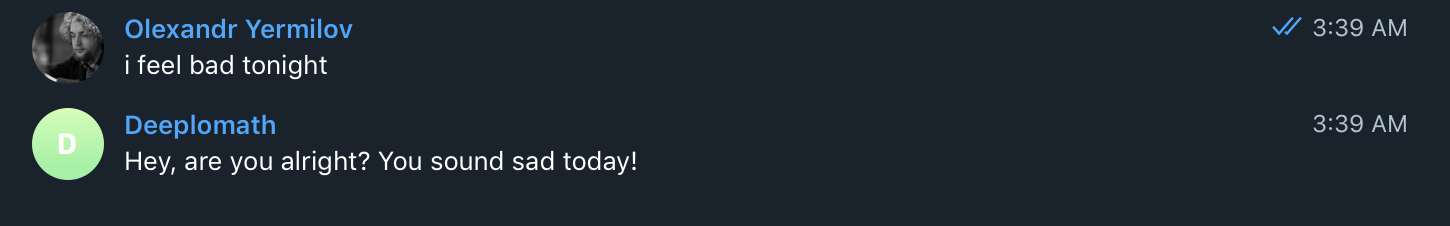
\includegraphics[width=500]{Dissertation/bad_sent.png}.\\
\textit{рис. 18. Приклад реакції на поганий настрій користувача.}

На прикладах, зображених на рисунках 17 і 18 маємо оцінки тону 0.545 і -0.437 відповідно. Через це, бот реагує відповідним чином.

\subsection{Розпізнавання іменованих сутностей}
Розпізнавання іменованих сутностей є важливою задачею для персонального асистента [21]. На основі іменованих сутностей, що були згадані під час діалогу користувача з чат-ботом, можна дізнаватись про його інтереси, запам'ятовувати факти, що допоможуть у подальших відповідях на питання. \\

\includegraphics[width = 450]{Dissertation/ner_1.png}\\
\textit{рис. 19. Приклад розпізнавання персони}\\
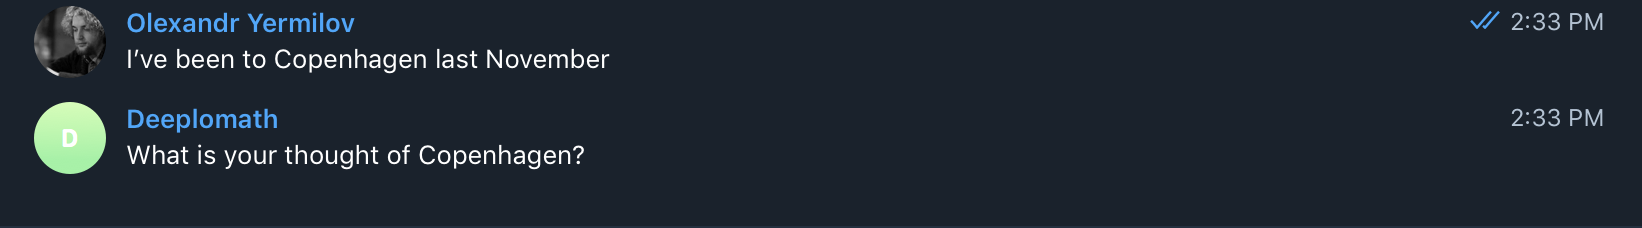
\includegraphics[width = 450]{Dissertation/ner_2.png}\\
\textit{рис. 20. Приклад розпізнавання локації}\\

Для розпізнавання іменованих сутностей використовувалась натренована модель з бібліотеки Spark NLP. Вона використовує word embeddings від моделі BERT. Спілкування між сервісом з Spark NLP та основною частиною боту відбувається за допомогою HTTP запитів.

В залежності від типу іменованої сутності, бот може задавати уточнюючі запитання. Також, бот може зберігати деякі з них як те, що пов'язане з користувачем або є сферою його інтересів.

Для покращення персоналізації, можемо час від часу запитувати про те, що було кваліфіковано як інтерес користувача. Це дозволить збирати більше даих, що в свою чергу дозволить покращувати роботу застосунку.
\subsection{Відповіді на питання}
Будемо зберігати усі повідомлення користувача, що були класифіковані як факти. 
Якщо ми кваліфікували деяке повідомлення від користувача як запитання, скористаємося моделлю BERT для того, щоб дати відповідь на нього. \\
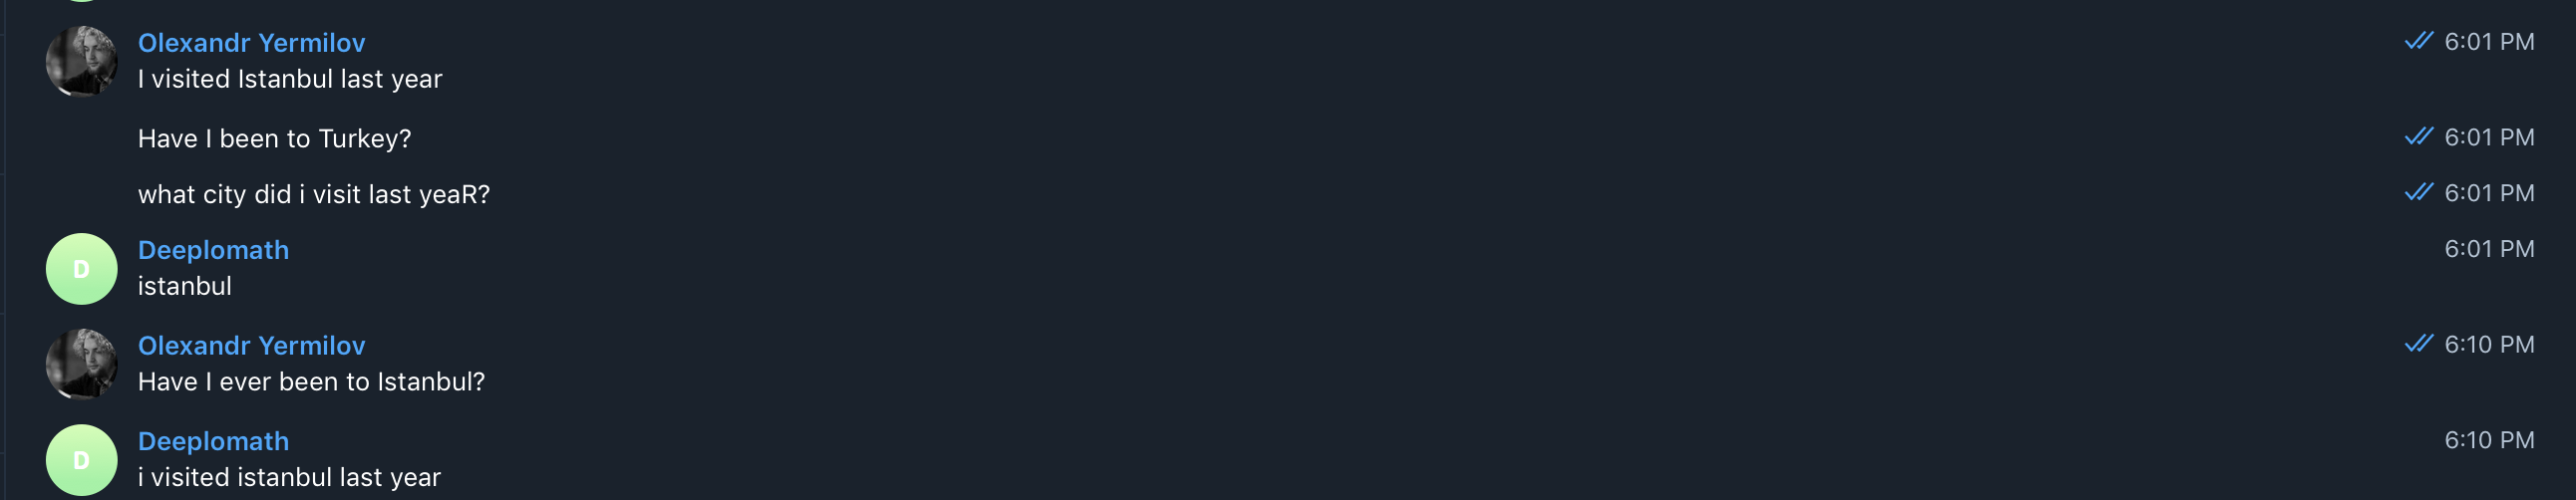
\includegraphics[width = 500]{Dissertation/bert_another.png}\\
\textit{рис 21. Відповіді на запитання користувача}.\\
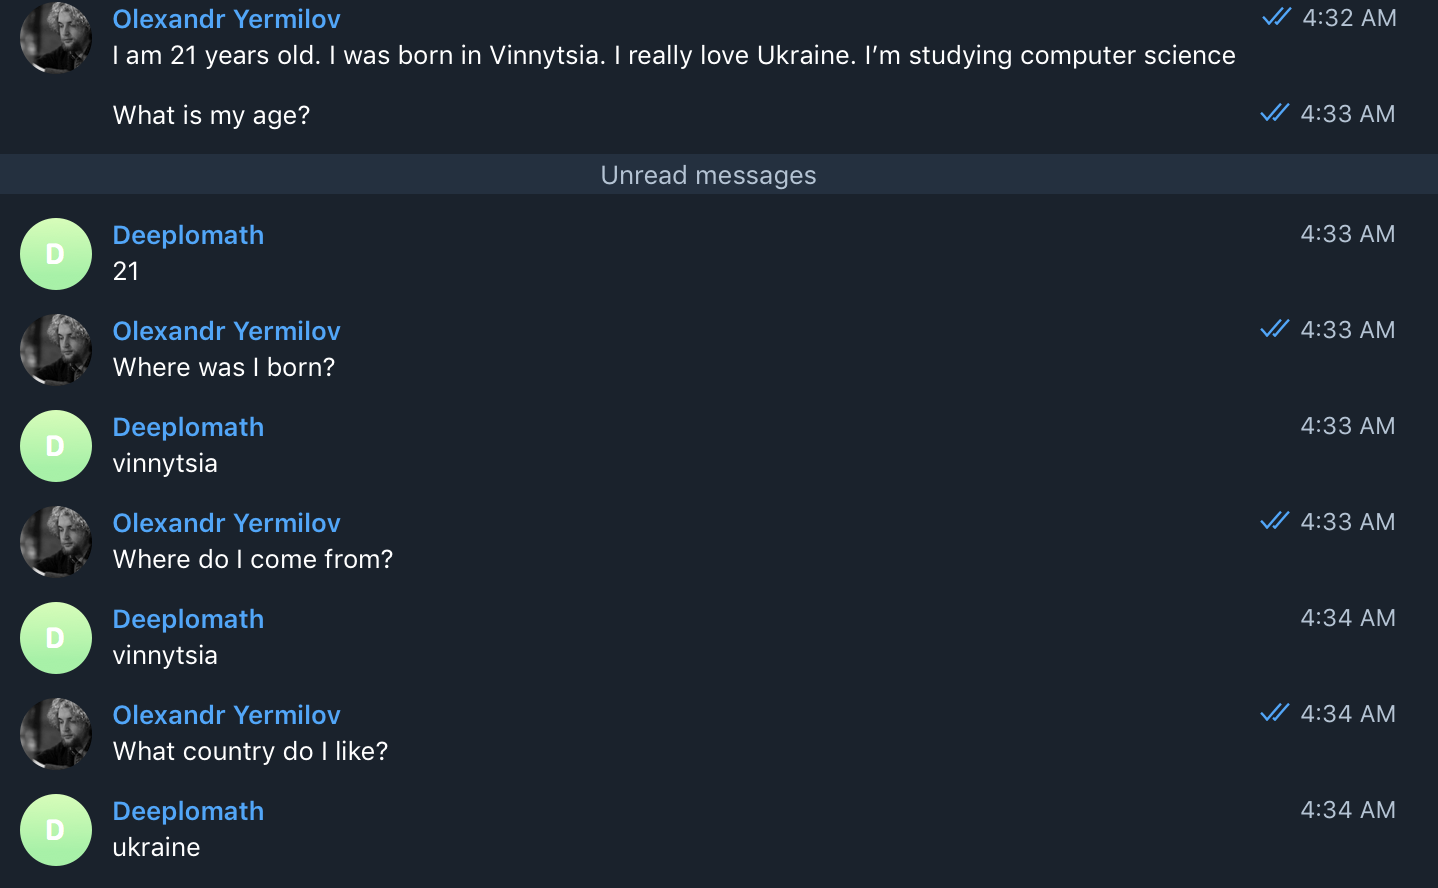
\includegraphics[width=500]{Dissertation/Bert_Example_1.png}.\\
\textit{рис 22. Ще один приклад відповідей на запитання.}

У якості тексту подамо усі повідомлення користувача, що були класифіковані як факти. Окрім того, враховуючи те, що бот має можливість і сам задавати запитання до користувача, ми можемо дописувати до вихідного тексту факти, які ми знаємо про користувача. Якщо збирати інформацію не тільки від користувача, а і від наприклад його гаджету (геолокація, локальний час, тощо) - матимемо змогу додати і ці факти до тексту, яким буде послуговуватись модель при відповіді на питання.

Можемо також враховувати і сфери інтересів користувача, отримані з інших функціональностей бота. Взагалі, модель дуже зручно використовувати для внутрішніх завдань бота - таких, як парсинг запитів користувача, тощо.

Дана модель відповідає в середньому за 0,2 - 0,3 секунди. Такий великий час відповіді пов'язаний з тим, що модель використовується без CUDA, що могло б значно пришвидшити роботу програми. Часом модель значно сповільнюється, на що також необхідно звернути увагу. 
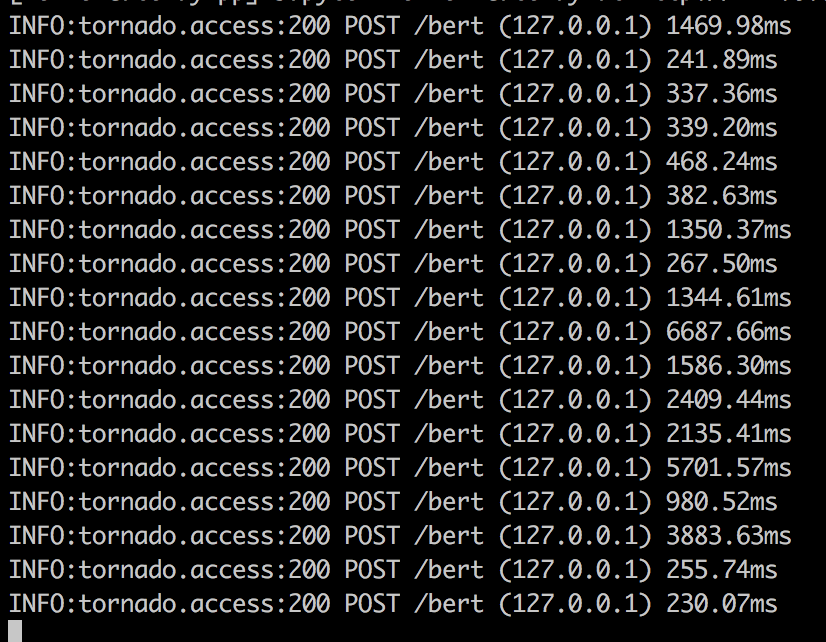
\includegraphics[height = 12cm]{Dissertation/bert_times.png}\\
\textit{рис. 23. Час роботи моделі на деяких запитаннях. }

Також дещо сповільнює роботу той факт, що спілкування між моделлю та серверною частиною застосунку відбувається через HTTP. Використання більш швидкого сервера для Python-частини могло би зменшити час, необхідний на відповідь.

BERT не має власної бази знань, і послуговується лише тим текстом, що був наданий користувачем. Таким чином, модель не може відповісти більшою кількістю інформації, ніж є у повідомленнях користувача. Як приклад, бачимо, що на рисунку 21 модель не може пов'язати Стамбул і Туреччину. Цю проблему можна вирішити якщо до кожного тексту, що надається для відповіді на питання, додавати базовий набір фактів з відкритих джерел про те, про що питає користувач.  Але з іншого боку, збільшення тексту збільшить час на обробку запитання. Також, можемо зробити свою базу знань, що дозволить відповідати на більш загальні питання користувача. В комбінації з розпізнаваннням теми повідомлення, ми можемо підключати бази знань що стоусуються заданої теми - і відповідати на ці питання.

Таку частину боту, що може відповідати на питання можна використовувати для витягнення короткого підсумку користувачем з тексту.




